% !TEX encoding = UTF-8
\documentclass[a4paper,12pt]{article}
\usepackage[T1]{fontenc}
\usepackage[utf8]{inputenc}
\usepackage[italian]{babel}
\usepackage{color, colortbl}
\usepackage{graphicx}
\definecolor{Ash}{rgb}{0.7,0.75,0.71}
\definecolor{Ash}{rgb}{0.7,0.75,0.71}
\definecolor{Ash}{rgb}{0.7,0.75,0.71}
\definecolor{Ash}{rgb}{0.7,0.75,0.71}
\usepackage{multirow}



\begin{document}

\title{\textbf{TrackMyCar - Live Positioning System}\\Project Plan}

\author{Kevin Mansoldo, Matteo Dal Monte, Luca Vicentini}
\date{}
\maketitle
\pagebreak

\tableofcontents
\pagebreak

\section{Lista Destinatari del Documento}

\begin{table*}[ht]
\begin{center}
\begin{tabular}{p{1cm} p{4.5cm} p{5cm} p{2cm}}
\rowcolor{Ash}
\hline
Copia & Persona & Organizzazione & Data \\ \hline
1 & Kevin Mansoldo & Azienda & Data \\ 
2 & Matteo Dal Monte & Azienda & Data \\ 
3 & Luca Vicentini & Azienda & Data \\ 
4 & Claudio Tomazzoli & Cliente & Data \\ \hline
\end{tabular}
\end{center}


\begin{center}
\begin{tabular}{p{6cm} p{5cm} p{2cm}}
\rowcolor{Ash}
\hline
Azione & Persona & Data \\ \hline
Documento redatto da & Kevin Mansoldo & Data \\ 
Documento approvato da & Matteo Dal Monte & Data \\ 
Documento approvato da & Luca Vicentini & Data \\ \hline
\end{tabular}
\end{center}
\end{table*}

\subsection{Versione Documento}
\begin{table*}[ht]
\begin{center}
\begin{tabular}{p{1cm} p{4.5cm} p{5cm} p{2cm}}
\rowcolor{Ash}
\hline
Versione & Autore & Note & Data \\ \hline
1.0 & Kevin Mansoldo & Stesura Iniziale & Data \\ 
1.1 & Kevin Mansoldo & Revisione su osservazioni del gruppo & Data \\ 
1.2 & Kevin Mansoldo & Revisione Finale & Data \\ \hline
\end{tabular}
\end{center}
\end{table*}

\subsection{Supporto Documento}
\begin{table*}[ht]
\begin{center}
\begin{tabular}{p{6cm} p{5cm} p{2cm}}
\rowcolor{Ash}
\hline
Nome File & Tipo & Estensione \\ \hline
ProjectPlan & Portable Document Format & .pdf \\ \hline
\end{tabular}
\end{center}
\end{table*}

\clearpage

\pagebreak

\section{Introduzione e Obiettivi}

Lo scopo del sistema che si vuole implementare è quello di poter tracciare in tempo reale il o i veicoli collegati in caso di furto o smarrimento. Tramite un'interfaccia visuale è possibile tenere sotto controllo la posizione, la velocità e lo storico dei percorsi effettuati. Inoltre viene fornita la possibilità di sfruttare l'integrazione con sistemi di videosorveglianza interni al veicolo, identificando così eventuali malintenzionati. 

L'applicazione, dotata di una intuitiva interfaccia grafica, permette quindi la rapida fruizione dei contenuti tramite semplici menu contestuali.


\section{Definizioni, Acronimi e Abbreviazioni}

Per le definizioni di alcuni termini fondamentali, fare riferimento al glossario ``Glossario.pdf'' all'interno della documentazione di progetto.

\begin{table}[h]
\begin{center}
\begin{tabular}{ p{4.5cm} p{4.5cm} p{3.5cm} } 
\rowcolor{Ash}	
\hline	
Nome File & Tipo File & Estensione  \\ \hline
Development Case & Linee guida di sviluppo del progetto & DevCase.pdf  \\ 
Glossario & Descrizione di termini specifici & Glossario.pdf  \\ 
Vision & Requisiti di sistema, Business Needs e Motivazioni & Vision.pdf  \\ 
Caratteristiche & Requisiti funzionali, non funzionali ed architetturali & Caratteristiche.pdf  \\ \hline
\end{tabular}
\end{center}
\end{table}

\pagebreak

\section{Organizzazione di Progetto}
\subsection{Componenti}
Il progetto vede l'utilizzo, per la creazione del prototipo nominato TrackMyCar by MadBox s.r.l., di svariate tecnologie che lo rendono appetibile e costantemente al passo con i tempi.
\subsection{Attività}
Nel progetto verranno affrontate le seguenti attività:
\begin{itemize}
\item Documentazione di Progetto
\begin{itemize}
\item Analisi dei Requisiti
\item Gestione Tecnica del Progetto
\end{itemize}
\item Database
\begin{itemize}
\item Progettazione 
\item Popolamento
\end{itemize}
\item Applicazione Web
\begin{itemize}
\item Logica applicativa
\item Interfaccia utente
\end{itemize}
\item Realizzazione modulo HW e installazione
\item Test
\end{itemize}

\pagebreak

\subsection{Matrice di Responsabilità}
\begin{table}[ht]
\begin{center}
\begin{tabular}{l | l | l | l}
\rowcolor{Ash}
\hline
\multicolumn{1}{ c |}{\multirow{2}{*}{Attività}}      & \multicolumn{3}{c}{Ruoli} \\ \cline{2-4}
\rowcolor{Ash}
  							    & Mansoldo & Dal Monte & Vicentini \\ \hline
 Documentazione di progetto & R & C & A \\ \hline
 Progettazione Database	    & A & R & C \\ \hline
 Popolamento Database	    & I  & R & A \\ \hline
 Logica Applicativa webapp   & A & C & R \\ \hline
 Interfaccia Utente			    & C & A & R \\ \hline
 Realizzazione Modulo HW   & I  & R &  A \\ \hline
 Manuale Utente			    & R & A & C \\ \hline
 Test						    & R & R & A \\ 
\hline
\end{tabular}
\end{center}
\end{table}

\begin{table}[ht]
\begin{center}
\begin{tabular}{c | c}
\rowcolor{Ash}
\hline
Lettera & Ruolo \\ \hline
R & Responsible \\
A & Accountable \\
C & Consulted \\
I  & Informed \\ \hline
\end{tabular}
\end{center}
\end{table}

\pagebreak

\subsection{Reticolo precedenze}
\begin{table}[ht]
\begin{center}
\begin{tabular}{c | c | c | c | c | c}
\rowcolor{Ash}
\hline
Milestone & Codice & Attività   					     & Durata & Predecessore & Successore \\ \hline
Inizio        & 	      &  		    					     &  		 &  				  &  \\ \hline
& & & & & PrDB \\
& Docs & Documentazione di Progetto & 7 & Inizio & LogA \\
& & & & & IntU \\
& & & & & ReHW \\ \hline
& PrDB     & Progettazione Database	    & 3 & Docs & PoDB \\ \hline
& PoDB    & Popolamento Database	    & 1 & PrDB & Test \\ \hline
& LogA     & Logica Applicativa webapp   & 10 & Docs & Test \\ \hline
& IntU       & Interfaccia Utente			    & 8 & Docs & ManU \\ 
& & & & & Test \\ \hline
& ReHW   & Realizzazione Modulo HW   & 5 & Docs & Test \\ \hline
& ManU    & Manuale Utente			    & 1 & IntU & Fine \\ \hline
& & & & PoDB & \\
& Test       & Test						    & 3  & LogA & Fine \\ 
& & & & IntU & \\
& & & & ReHW & \\ \hline
Fine && 						    &  &  &  \\
\hline
\end{tabular}
\end{center}
\end{table}
\pagebreak

\subsection{Percorso Critico}
\begin{figure}[htbp]
\centering
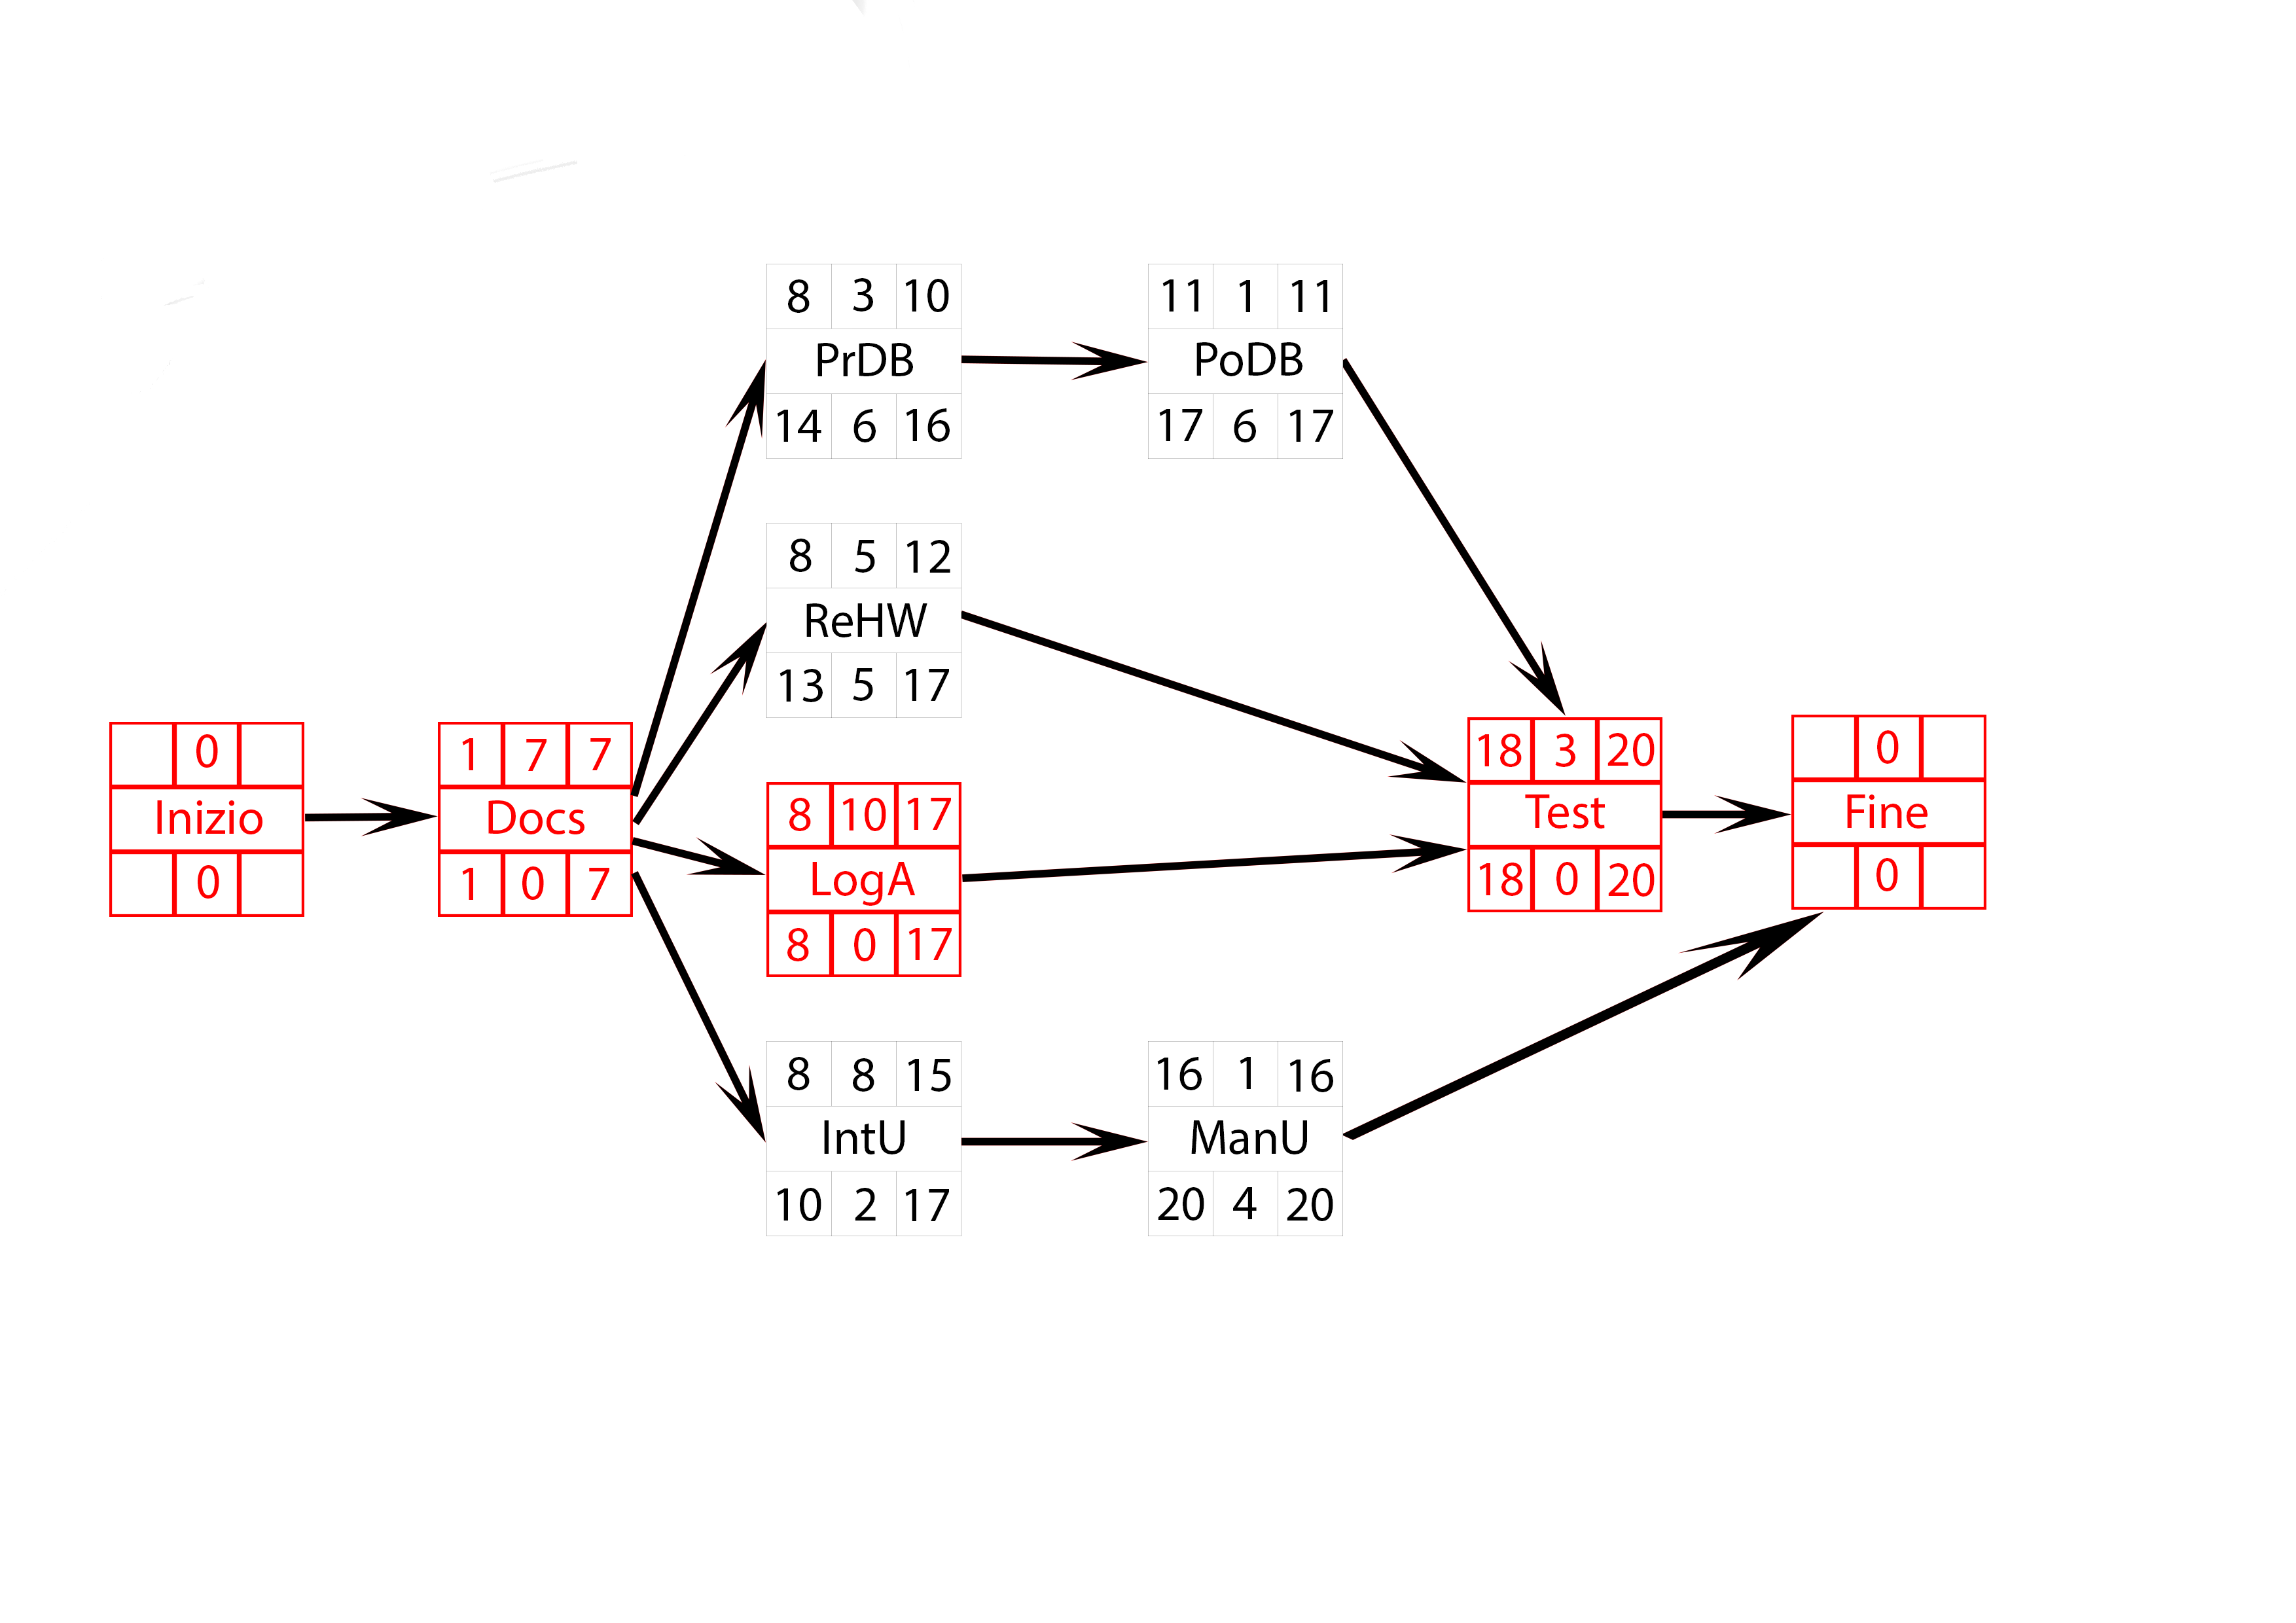
\includegraphics[trim={1cm 4.5cm 3.5cm 2.5cm}, clip, scale=0.6]{CPM.png}
\end{figure}

\section{Rilascio Deliverables}
Il completamento delle attività sovrastanti produrrà i seguenti deliverables:
\begin{itemize}
\item Database su cui verranno salvati i dati ricevuti dal modulo di Track~My~Car
\item La centralina Hardware da installare fisicamente sul veicolo
\item Webapp di gestione del modulo (JSP)
\item Documentazione a supporto (Manuale Utente)
\end{itemize}
\pagebreak

\section{Cronoprogramma}
\begin{figure}[htbp]
\centering
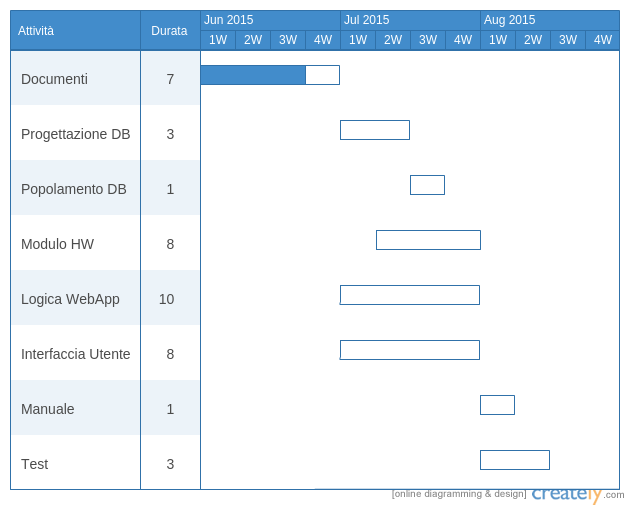
\includegraphics[trim={0 0.66cm 0 0}, clip, scale=0.5]{gantt.png}
\end{figure}
\begin{table}[ht]
\begin{center}
\begin{tabular}{l | l | l}
\rowcolor{Ash}
\hline
Data Inizio        & Data Fine	      &  	Oggetto	     \\ \hline
01/06/2015 & 30/06/2015 & Documentazione di progetto  \\ \hline
01/07/2015 & 10/07/2015 & Progettazione Database	     \\ \hline
11/07/2015 & 12/07/2015 & Popolamento Database	     \\ \hline
11/07/2015 & 20/07/2015 & Realizzazione Modulo HW    \\ \hline
10/07/2015 & 10/08/2015 & Logica Applicativa webapp    \\ \hline
10/07/2015 & 10/08/2015 & Interfaccia Utente			     \\ \hline
11/08/2015 & 12/08/2015 & Manuale Utente			     \\ \hline
19/08/2015 & 10/09/2015 & Test						     \\ 
\hline
\end{tabular}
\end{center}
\end{table}
\end{document}